%% ------------------------------------------------------------------------- %%
\chapter{Experimentos}
\label{cap:experimentos}

Este capítulo é dividido em quatro seções. Primeiro, na Seção
\ref{sec:powerworkflowsim} é comentada a tentativa de implementação de um
simulador, o PowerWorkflowSim para os experimentos realizados nesta monografia.
Depois, na Seção \ref{sec:ambiente_simulado} são apresentados os parâmetros
utilizados nas simulações desenvolvidas. Em seguida, na Seção
\ref{sec:fluxos_trabalho} são apresentados três fluxos de trabalho que servirão
como dados de entrada para os algoritmos de escalonamento. Por fim, na Seção
\ref{sec:resultados_experimentais} são apresentados os resultados experimentais
e uma comparação com os algoritmos de referência escolhidos.

% Este capítulo é dividido em quatro momentos distintos dos experimentos realizados
% para esta monografia. Primeiro, na Seção \ref{sec:powerworkflowsim} é
% apresentado o simulador desenvolvido para esta monografia, o PowerWorkflowSim;
% Depois, na Seção \ref{sec:ambiente_simulado} são
% apresentadas as configurações do ambiente experimental; Resultados dos 
% experimentos de controle são exibidos na Seção \ref{sec:experimentos-controle}.
% Em seguida, na Seção
% \ref{sec:algoritmo_proposto} é feito um estudo detalhado sobre a heurística
% proposta para minimizar o consumo energético e o algoritmo correspondente
% implementado; Por fim na Seção \ref{sec:resultados_experimentais} são
% apresentados os resultados experimentais que mostram o ganho energético com
% o uso do algoritmo proposto.

\section{PowerWorkflowSim}
\label{sec:powerworkflowsim}

Durante a implementação do WorkflowSim os desenvolvedores não tomaram o cuidado
de manter a API de simulação energética do CloudSim acessível ao usuário final.
De maneira a resolver esse problema, o autor da monografia tentou desenvolver
uma versão alternativa do WorkflowSim, o PowerWorkflowSim.

Tanto a API energética do CloudSim quanto o WorkflowSim fazem intenso uso de
herança de objetos para reaproveitamento de código e funcionalidades
semelhantes. Isto é evidenciado na Figura \ref{fig:classes_simuladores}, que
agrupa um subconjunto das classes principais dos simuladores estudados e suas
relações.

Como Java, a linguagem na qual os simuladores foram desenvolvidos, não possui
suporte a herança múltipla a estratégia empregada foi a de criar classes
herdadas da API energética (\texttt{PowerDatacenter} e \texttt{PowerVm}, etc) e
reimplementar as mudanças propostas pelo WorkflowSim
(\texttt{DatacenterExtended} e \texttt{CondorVm}, etc) nestas novas
classes (\texttt{PowerDatacenterExtended} e \texttt{PowerCondorVm}, etc).

Porém, após três semanas de trabalho lento e minucioso analisando \emph{traces}
da execução do simulador não foi possível chegar a um código estável, no qual
uma implementação não conflitasse com outra. Com a disponibilização
do código fonte do CloudSim\_DVFS o projeto de desenvolver o PowerWorkflowSim
foi abandonado.

Vale ressaltar que em conversa com o desenvolvedor do CloudSim\_DVFS foi
possível descobrir que ele também enfrentou os mesmos problemas, tendo que
recorrer a caminhos alternativos para desenvolver o seu simulador. As
dificuldades enfrentadas por ele foram apresentadas aos desenvolvedores do
CloudSim mas estes ainda não identificaram onde aconteceu o problema.

Outro fato relevante a ser notado é que apesar do WorkflowSim não ter sido
utilizado como simulador, foram feitas contribuições ao código do simulador.
Um \emph{pull request} contendo a implementação do algoritmo HEFT foi aceita
para incorporação no repositório do simulador. Ainda, o autor da monografia
foi aceito como contribuidor no projeto.

\begin{figure}[ht]
\centering
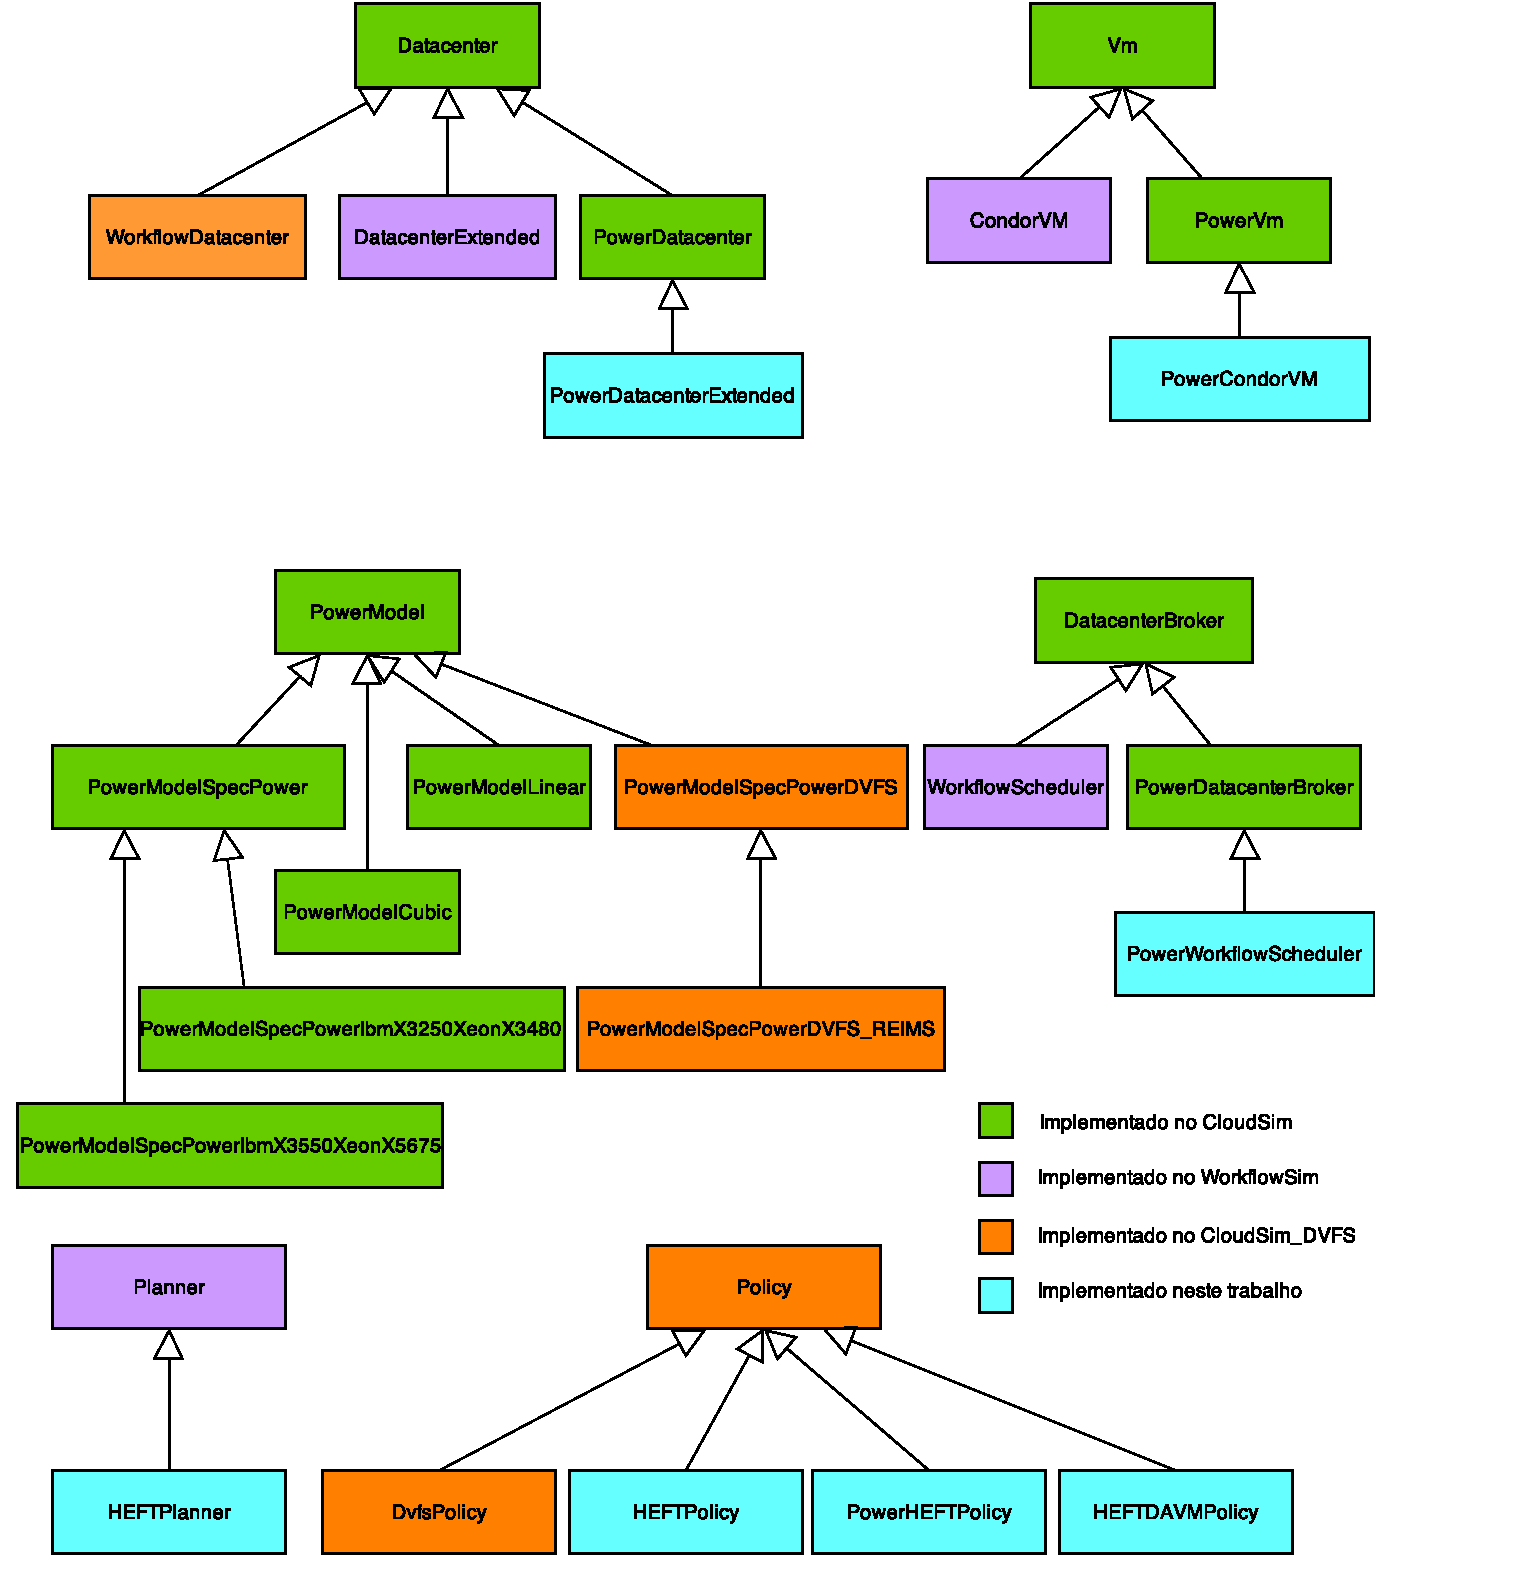
\includegraphics[width=\textwidth]{ClassesSimuladores.pdf}
\caption{Diagrama de classes dos simuladores estudados}
\label{fig:classes_simuladores}
\end{figure}

\section{Ambiente Simulado}
\label{sec:ambiente_simulado}

O ambiente simulado foi o mesmo que o artigo
\cite{guerout:energy_aware_simulation} utilizou em seus experimentos e é baseado
no Grid'5000 REIMS \cite{cappello:grid5000}. As configurações utilizadas estão
descritas na Tabela \ref{tab:configuracoes_cloudsim_dvfs}.

\begin{table}
	\centering
    \begin{tabular}{c|c}
    \hline
    \textbf{Configuração}                     & \textbf{Valor}                                   \\ \hline
    Número de máquinas físicas (\emph{hosts}) & 500                                              \\
    Atraso na inicialização de uma VM         & 120 ms                                           \\
    Tipos de VMs disponíveis                  & Descrito na seção \ref{sec:modelagem_energetica} \\
    Número de núcleos por \emph{host}         & 8                                                \\
    RAM por \emph{host}                       & 32 GB                                            \\
    Espaço em disco por \emph{host}           & 10 TB                                            \\
    Frequência de cada núcleo                 & 1000 MIPS                                        \\
    Latência da rede                          & 0.2 ms                                           \\
    Latência interna                          & 0.05 ms                                          \\
    Largura de banda                          & 1250 Mbps                                        \\ \hline
    \end{tabular}
    \caption{Configurações do ambiente simulado}
    \label{tab:configuracoes_cloudsim_dvfs}
\end{table}


\section{Fluxos de Trabalho Utilizados}
\label{sec:fluxos_trabalho}

Para facilitar a análise de algoritmos que operam sobre fluxos de trabalho,
tais como os algoritmos descritos nesta monografia, o projeto Pegasus Workflow
Management System desenvolveu uma ferramenta geradora de \emph{workflows}
científicos. Estes \emph{workflows} artificiais são gerados a partir de
informações extraídas de instâncias reais das aplicações juntamente com
conhecimentos prévios sobre seu funcionamento interno
\cite{pegasus:workflowgenerator}. 

\begin{figure}
        \centering
        \begin{subfigure}[b]{0.3\textwidth}
                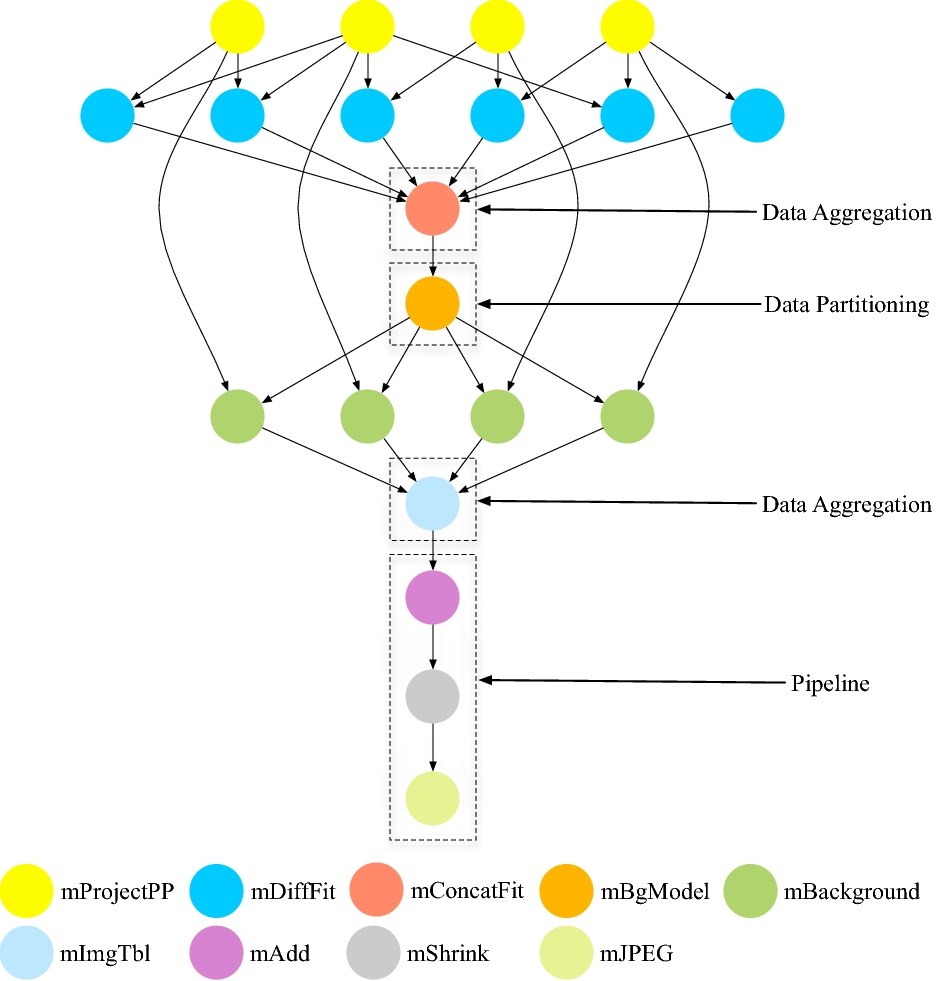
\includegraphics[width=\textwidth]{Montage.jpg}
                \caption{A aplicação Montage, criada pela NASA/IPAC agrupa
                diversas imagens de entrada para gerar mosaicos personalizados
                do céu.}
                \label{fig:montage}
        \end{subfigure}%
        ~ %add desired spacing between images, e. g. ~, \quad, \qquad etc.
          %(or a blank line to force the subfigure onto a new line)
        \begin{subfigure}[b]{0.3\textwidth}
                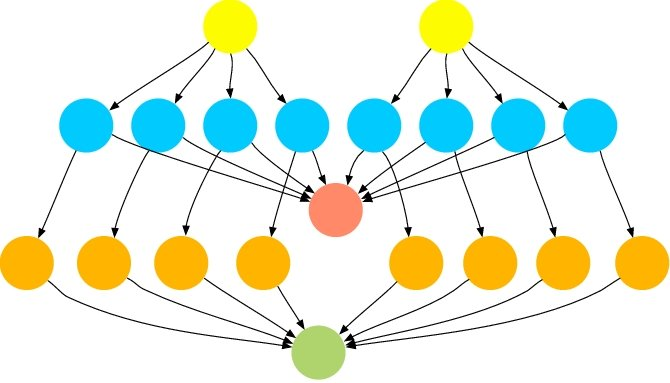
\includegraphics[width=\textwidth]{CyberShake.jpg}
                \caption{A aplicação CyberShake é usada pelo Centro de Terremotos
                do Sul da Califórnia para caracterizar riscos de terremotos em uma
                região.}
                \label{fig:cybershake}
        \end{subfigure}
        ~
        \begin{subfigure}[b]{0.3\textwidth}
                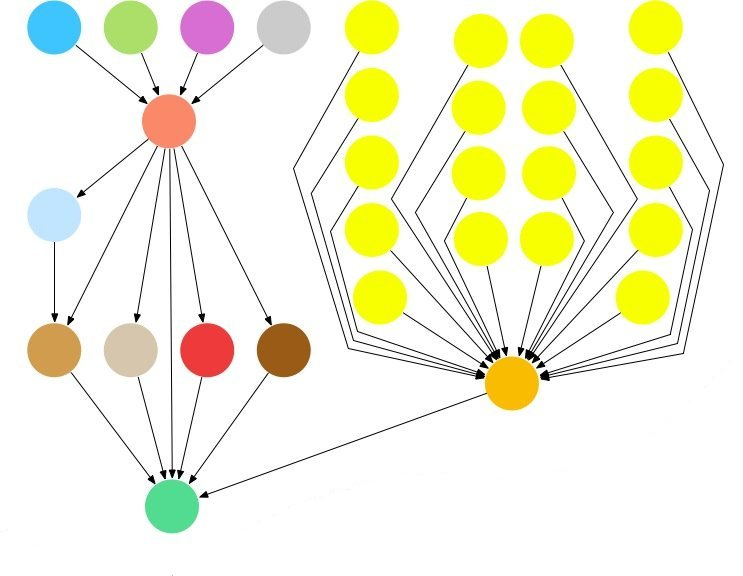
\includegraphics[width=\textwidth]{Sipht.jpg}
                \caption{A aplicação Sipht foi criada pela Universidade de
                Harvard para automatizar a busca por RNAs não traduzidos (sRNAs)
                em um banco de dados.}
                \label{fig:sipht}
        \end{subfigure}%
        \caption{Exemplos de DAGs das aplicações simuladas. Imagens retiradas
        do Projeto Pegasus, sob a licença Apache.}
        \label{fig:dags_aplicacoes}
\end{figure}


Os fluxos gerados pelo projeto Pegasus são então executados no CloudSim\_DVFS
com as configurações apresentadas na Seção \ref{sec:ambiente_simulado}. É
importante notar a necessidade de realizar testes com fluxos de trabalho com
diferentes topologias. Alguns algoritmos de escalonamento podem ser mais
adequados a fluxos de trabalho mais ou menos paralelos.


\section{Resultados Experimentais}
\label{sec:resultados_experimentais}

Os resultados extraídos das simulações feitas com os três fluxos de trabalho
descritos na Seção \ref{sec:fluxos_trabalho} estão descritos abaixo. São feitas
análises tanto do consumo energético quanto do tempo de conclusão de cada
aplicação (\emph{makespan}). A Figura \ref{fig:graficos_aplicacoes} resume esta
seção, com os gráficos de uso de energia e tempo para cada um dos
\emph{workflows}.


\subsection{Sipht}
\label{sec:sipht}

As Tabelas \ref{tab:sipht_tempo} e \ref{tab:sipht_energia} apresentam o
\emph{makespan} e o consumo energético respectivamente da aplicação Sipht para
todos os algoritmos de escalonamento testados. Neste caso, todos os algoritmos
conseguiram superar o modo de referência, Performance para a instância de 30
vértices. No entanto, entradas maiores mostram que o modo OnDemand é mais
eficiente para este fluxo de trabalho. A economia energética foi de 15\% para a
instância com 100 vértices. Já os \emph{makespans} desta instância, exceto o
PowerHEFT, estão distribuídos na faixa de [1957 - 2501] segundos.

Ainda, a estratégia de \emph{clustering} (Algoritmos DAVM-TC e Optimal-TC)
mostraram-se vantajosos superando a eficiência em ambos os critérios de suas
versões regulares.

\begin{table}
	\centering
    \begin{tabular}{c|ccc}
    ~                    & Sipht\_30 & Sipht\_60 & Sipht\_100 \\ \hline
    Performance (Sem DVFS)                              & 2349     & 1975     & 1957      \\
    \cite{guerout:energy_aware_simulation} Optimal      & 2349     & 2249     & 2176      \\
    \cite{guerout:energy_aware_simulation} OnDemand     & 2349     & 1975     & 1957      \\
    HEFT                                                & 2327     & 2443     & 2367      \\
    PowerHEFT                                           & 4016     & 16330    & 40239     \\
    DAVM                                                & 2340     & 2500     & 2501      \\
    DAVM-TC                                             & 2340     & 2500     & 2501      \\
    Optimal-TC                                          & 2324     & 2179     & 2162      \\
    \end{tabular}
    \caption{\emph{Makespan} calculado para a aplicação Sipht}
    \label{tab:sipht_tempo}
\end{table}



\begin{table}
	\centering
    \begin{tabular}{r|ccc}
    ~                    & Sipht\_30 & Sipht\_60 & Sipht\_100 \\ \hline
    Performance (Sem DVFS) & 3241     & 5484     & 9060      \\
    \cite{guerout:energy_aware_simulation} Optimal      & 2818     & 5373     & 8648      \\
    \cite{guerout:energy_aware_simulation} OnDemand     & 2751     & 4669     & 7702      \\
    HEFT                   & 3211     & 6745     & 10904     \\
    PowerHEFT              & 2925     & 6006     & 8886      \\
    DAVM                   & 2860     & 6172     & 10217     \\
    DAVM-TC                & 2858     & 6116     & 10166     \\
    Optimal-TC             & 2784     & 5205     & 8590      \\
    \end{tabular}
    \caption{Consumo energético calculado para a aplicação Sipht}
    \label{tab:sipht_energia}
\end{table}


\subsection{CyberShake} % (fold)
\label{sub:cybershake}

As Tabelas \ref{tab:cybershake_tempo} e \ref{tab:cybershake_energia} apresentam o
\emph{makespan} e o consumo energético respectivamente da aplicação CyberShake para
todos os algoritmos de escalonamento testados. Aqui, o comportamento foi similar
ao Sipht. Os escalonadores propostos foram eficientes em entradas pequenas mas
perderam para o algoritmo OnDeman na comparação com entradas maiores. Novamente
o \emph{clustering} se mostrou uma boa otimização em um algoritmo de
escalonamento.


\begin{table}
	\centering
    \begin{tabular}{c|ccc}
    ~                    & CyberShake\_30 & CyberShake\_50 & CyberShake\_100 \\ \hline
    Performance (Sem DVFS) & 265           & 271           & 271            \\
    \cite{guerout:energy_aware_simulation} Optimal      & 272           & 271           & 271            \\
    \cite{guerout:energy_aware_simulation} OnDemand     & 265           & 271           & 271            \\
    HEFT                   & 332           & 245           & 417            \\
    PowerHEFT              & 753           & 2175          & 8421           \\
    DAVM                   & 263           & 406           & 453            \\
    DAVM-TC                & 261           & 365           & 436            \\
    Optimal-TC             & 257           & 271           & 273            \\
    \end{tabular}
    \caption{\emph{Makespan} calculado para a aplicação CyberShake}
    \label{tab:cybershake_tempo}
\end{table}



\begin{table}
	\centering
    \begin{tabular}{l|lll}
    ~                    & CyberShake\_30 & CyberShake\_50 & CyberShake\_100 \\ \hline
    Performance (Sem DVFS) & 380           & 651           & 1305           \\
    \cite{guerout:energy_aware_simulation} Optimal      & 352           & 636           & 1210           \\
    \cite{guerout:energy_aware_simulation} OnDemand     & 323           & 555           & 1114           \\
    HEFT                   & 473           & 823           & 1982           \\
    PowerHEFT              & 533           & 928           & 1805           \\
    DAVM                   & 358           & 908           & 2012           \\
    DAVM-TC                & 351           & 803           & 1900           \\
    Optimal-TC             & 330           & 636           & 1217           \\
    \end{tabular}
    \caption{Consumo energético calculado para a aplicação CyberShake}
    \label{tab:cybershake_energia}
\end{table}
% subsection cybershake (end)



\subsection{Montage} % (fold)
\label{sub:montage}

Já para a aplicação Montage, os resultados foram diferentes. Os escalonadores
baseados no HEFT se mostraram melhores que os propostos por
\cite{guerout:energy_aware_simulation}, inclusive superando o modo OnDemand.
Neste caso, \emph{clustering} não trouxe ganhos significativos em tempo ou
energia.

\begin{table}
	\centering
    \begin{tabular}{c|ccc}
    ~                    & Montage\_25 & Montage\_50 & Montage\_100 \\ \hline
    Performance (Sem DVFS) & 205        & 231        & 236         \\
    \cite{guerout:energy_aware_simulation} Optimal      & 205        & 231        & 236         \\
    \cite{guerout:energy_aware_simulation} OnDemand     & 205        & 231        & 236         \\
    HEFT                   & 174        & 179        & 188         \\
    PowerHEFT              & 262        & 419        & 732         \\
    DAVM                   & 180        & 195        & 189         \\
    DAVM-TC                & 177        & 195        & 183         \\
    Optimal-TC             & 205        & 231        & 236         \\
    \end{tabular}
    \caption{\emph{Makespan} calculado para a aplicação Montage}
    \label{tab:montage_tempo}
\end{table}



\begin{table}
	\centering
    \begin{tabular}{c|ccc}
    ~                      & Montage\_25 & Montage\_50 & Montage\_100 \\ \hline
    Performance (Sem DVFS) & 241        & 544        & 1111        \\
    \cite{guerout:energy_aware_simulation} Optimal      & 241        & 544        & 1111        \\
    \cite{guerout:energy_aware_simulation} OnDemand     & 204        & 459        & 938         \\
    HEFT                   & 206        & 423        & 889         \\
    PowerHEFT              & 307        & 980        & 3412        \\
    DAVM                   & 200        & 436        & 817         \\
    DAVM-TC                & 195        & 438        & 784         \\
    Optimal-TC             & 205        & 544        & 1111        \\
    \end{tabular}
    \caption{Consumo energético calculado para a aplicação Montage}
    \label{tab:montage_energia}
\end{table}
% subsection montage (end)

\begin{figure}
        \centering
        \begin{subfigure}[b]{0.5\textwidth}
                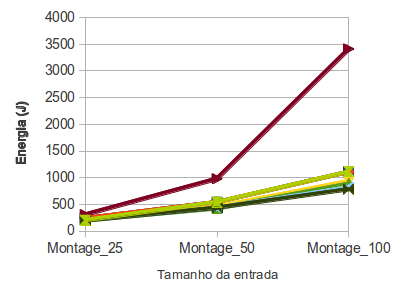
\includegraphics[width=\textwidth]{montage_energia.png}
                \caption{Consumo energético da aplicação Montage}
                \label{fig:montage_energia}
        \end{subfigure}%
        ~ %add desired spacing between images, e. g. ~, \quad, \qquad etc.
          %(or a blank line to force the subfigure onto a new line)
        \begin{subfigure}[b]{0.5\textwidth}
                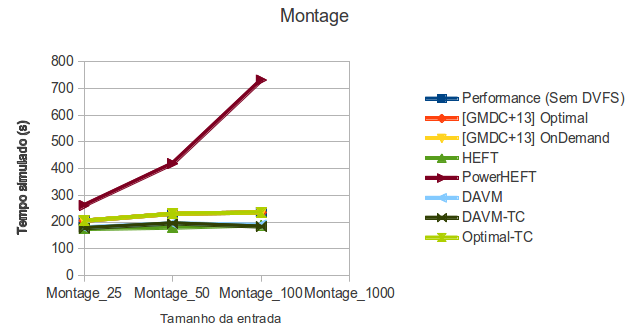
\includegraphics[width=\textwidth]{montage_tempo.png}
                \caption{\emph{Makespan} da aplicação Montage}
                \label{fig:montage_tempo}
        \end{subfigure}

        \begin{subfigure}[b]{0.5\textwidth}
                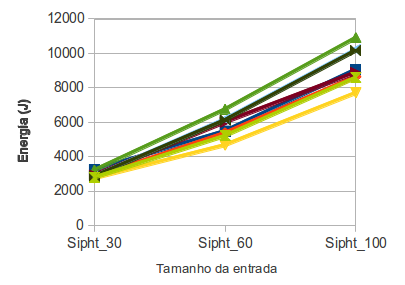
\includegraphics[width=\textwidth]{sipht_energia.png}
                \caption{Consumo energético da aplicação Sipht}
                \label{fig:sipht_energia}
        \end{subfigure}%
        ~ %add desired spacing between images, e. g. ~, \quad, \qquad etc.
          %(or a blank line to force the subfigure onto a new line)
        \begin{subfigure}[b]{0.5\textwidth}
                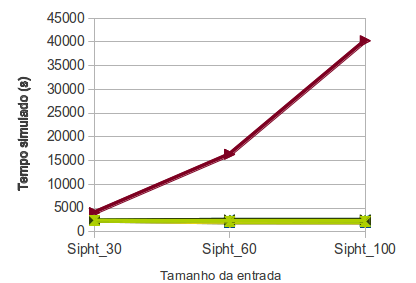
\includegraphics[width=\textwidth]{sipht_tempo.png}
                \caption{\emph{Makespan} da aplicação Sipht}
                \label{fig:sipht_tempo}
        \end{subfigure}

        \begin{subfigure}[b]{0.5\textwidth}
                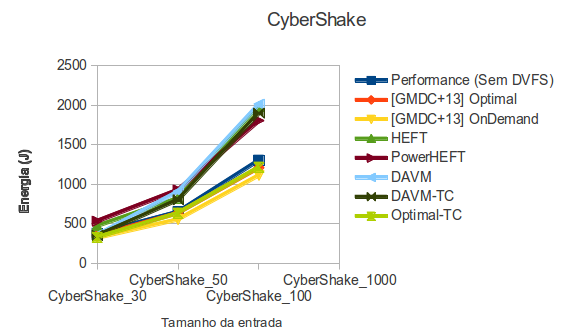
\includegraphics[width=\textwidth]{cybershake_energia.png}
                \caption{Consumo energético da aplicação CyberShake}
                \label{fig:cybershake_energia}
        \end{subfigure}%
        ~ %add desired spacing between images, e. g. ~, \quad, \qquad etc.
          %(or a blank line to force the subfigure onto a new line)
        \begin{subfigure}[b]{0.5\textwidth}
                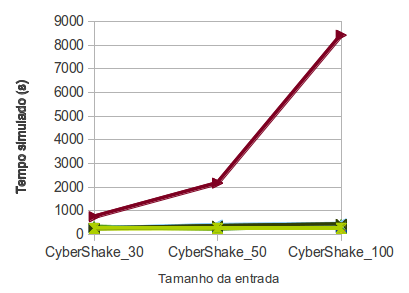
\includegraphics[width=\textwidth]{cybershake_tempo.png}
                \caption{\emph{Makespan} da aplicação CyberShake}
                \label{fig:cybershake_tempo}
        \end{subfigure}

        \begin{subfigure}[b]{0.25\textwidth}
                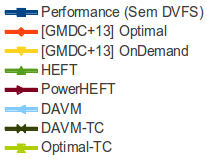
\includegraphics[width=\textwidth]{legenda.png}
                \caption{Legenda dos gráficos}
                \label{fig:legenda_graficos}
        \end{subfigure}%
        \caption{Gráficos do consumo energético e \emph{makespan} das aplicações
        Montage, Sipht e CyberShake.}\label{fig:graficos_aplicacoes}
\end{figure}

